\documentclass[12pt,a4paper]{report}
\usepackage{amsmath, amssymb, amsthm}
\usepackage{enumitem}
\usepackage{hyperref}
\usepackage{bm}
\usepackage[utf8]{inputenc}     % if you need it
\usepackage[T1]{fontenc}        % if you need it
% \usepackage{subcaption}         % defines the subfigure environment
\usepackage{grffile}
\usepackage{placeins}    
\usepackage[a4paper,margin=1in]{geometry}
\usepackage{graphicx}
\usepackage{subcaption}
\usepackage{booktabs}
\usepackage{float}       % for [H]
\usepackage{placeins}    % for \FloatBarrier


\hypersetup{
    colorlinks=true,
    linkcolor=black,
    urlcolor=black,
    citecolor=black
}

\begin{document}

\tableofcontents
\setcounter{chapter}{1}
\chapter{Part B}
%======================================
\section{Theoretical background}

% REPLACED theoretical background subsections 1-7 with new content:

\subsection{Newton’s Law of Cooling: Fundamentals}
Newton’s law of cooling asserts that the instantaneous rate of heat flow from a body to its surroundings is directly proportional to the temperature difference between them. Microscopically, this arises because the net energy exchanged per unit time depends on the frequency and energy of molecular collisions at the interface. Macroscopically, one writes
\begin{equation}
    \dot{Q} = -\,h\,A\,(T - T_E),
\end{equation}
where $\dot{Q} = \frac{dQ}{dt}$ is the heat flux from the body, $h$ the convective heat‐transfer coefficient, $A$ the exchange area, $T(t)$ the temperature of the body, and $T_E$ the ambient or environment temperature. The negative sign indicates that heat flows out when $T>T_E$.


 When heat is transferred at a low enough rate one can consider that the body remains nearly isothermal during cooling, and one may treat its entire heat content as lumped into a single thermal capacitance $C=m\,c_p$. Applying conservation of energy to the body yields the ordinary differential equation
\[
C\,\frac{dT}{dt} = -\,h\,A\,(T - T_E),
\]
which relates the time‐rate change of the body’s temperature to the net heat flux.

\subsection{Analytical Solution and Time Constant}
To solve the ODE eparation of variables is used,
\[
\frac{dT}{T - T_E} = -\,\frac{h\,A}{C}\,dt,
\]
and integrating from the initial temperature $T_0$ at $t=0$ gives an exponential decay law:

\begin{equation} \label{T_v_t_exponential}
    T(t) - T_E = (T_0 - T_E)\,\exp\!\bigl(-t/\tau\bigr),
\end{equation}

with characteristic time constant
\[
\tau = \frac{C}{h\,A}.
\]
Physically, $\tau$ represents the time required for the temperature difference to diminish by a factor of $1/e$.

\subsection{Two‐Path Cooling in Cup Experiments}
In our open‐cup experiment, the hot water loses heat both through the styrofoam walls and by direct convection at the free surface. Writing each path as a conductance, according to thermodynamics defines the total conductance as
\[
U_{\rm tot} = h_{\rm cup}\,A_{\rm cup} + h_{\rm air}\,A_{\rm air},
\]
so that the cooling follows $C_w\,\frac{dT}{dt} = -\,U_{\rm tot}(T-T_E)$ with time constant $\tau_1=C_w/U_{\rm tot}$. In the insulated cooling process where the water is only cooled from heat exchange with the cup, surface convection is suppressed and only the cup conductance remains, giving $\tau_2=C_w/(h_{\rm cup}A_{\rm cup})$. Subtracting the reciprocals,
\[
\frac1{\tau_1} - \frac1{\tau_2} = \frac{h_{\rm air}A_{\rm aur}}{C_w},
\]
allows us to isolate the air conductance.

\subsection{Parameter Extraction Procedure}
 In this expirement the tempreture $\Delta T$ is measured at equally spaced intervals of time. Plotting $\ln(\Delta T )$ versus $t$ yields a straight line, according to \eqref{T_v_t_exponential} it's slope equals $-1/\tau$. By fitting both open‐cup and insulated data sets, one extracts $\tau_1$ and $\tau_2$ and then determines
\begin{equation}
    h_{\rm cup}A_{\rm cup} = \frac{C_w}{\tau_2},\qquad
h_{\rm air}A_{\rm air} = C_w\Bigl(\tfrac1{\tau_1}-\tfrac1{\tau_2}\Bigr).
\end{equation}

Finally, dividing by known areas yields the heat transfer coefficients $h_{\rm cup}$ and $h_{\rm air}$.

%======================================
\section{Methodology}
\subsection{Experimental objective}
Confirmation of newton's cooling law.
\subsection{Materials}
\begin{itemize}[leftmargin=2em]
    \item Rod used for mixing.
    \item Electric kettle.
    \item Cup for hot water and system for dipping sensors.
    \item Thermal resistant lid.
    \item Temperature sensor PT-100 ($-200^\circ$C to $+400^\circ$C) with a resolution of $0.188[^\circ C]$, $1[sec]$.
    \item Multi-Log logger.
\end{itemize} 
\subsection{Experimental procedue}
\subsubsection{Part A}
First, to get ready for this part it is needed to measure the room temperature with the temperature sensor.
\newline
After that the electric kettle would be used to boil water. 
The water then would be put inside the fitting cup and the temperature probe lowered inside.
Then once a minute the temperatue of the water will be measured for as long as possible (at least one hour).
\subsubsection{Part B}
For this part part A will be repeated with the slight change of having a thermal resistant lid closing the cup.

\section{Data analysis process }
For the data processing it is first needed to fit the measured temperature in part b as a exponential function of the time with the next equation:
\begin{equation}
    y = a_0 + a_1\cdot e^{-a_2 x}
\end{equation}
Where $\Delta T$ was calculated from Expirament A:
$$\Delta T = 0.054 [^\circ C]$$
And from equation (28) in the data processing brochure:
$$\Delta t = 0.29 [sec]$$
From equation (\eqref{exp theo}) it is expected that:
$$a_{0,only cup} = 0[^\circ C]$$
From eqation (\eqref{exp theo}) it is expected that:
$$a_{2,only cup} = \frac{h\cdot A}{C_w}$$

After that from equation (\eqref{exp fit}) equation (\eqref{exp theo}) and equation (\eqref{b}) a fit of the temperatue measured in part A as a function of the time will be done:
From equation (\eqref{exp theo}) it is expected that:
$$a_{0,cup + water} = 0[^\circ C]$$
From eqation (\eqref{exp theo}) it is expected that:
$$a_{2, cup + water} = \frac{h\cdot A}{C_w}$$

And so $C_{w, theo}$ will be used in equation (\eqref{h_air A_air=...}) to find $h_{exp, avg}$:
\begin{equation}
    h = C_w(a_{2, cup+water}-a_{2, onlycup}) \pm C_w\sqrt{(\Delta a_{2, cup+water})^2+(\Delta a_{2, onlycup})^2}
\end{equation}
At last as $h(boil)\approx 20000$ and $h(room) \approx 0$ it is expected that h is in this range.


\pagebreak
\section{Data analysis}
After fitting the results to the exponential fit and extracting the parameter we got: 


\begin{figure}[htbp]
    \centering
    \begin{subfigure}[b]{0.48\textwidth}
      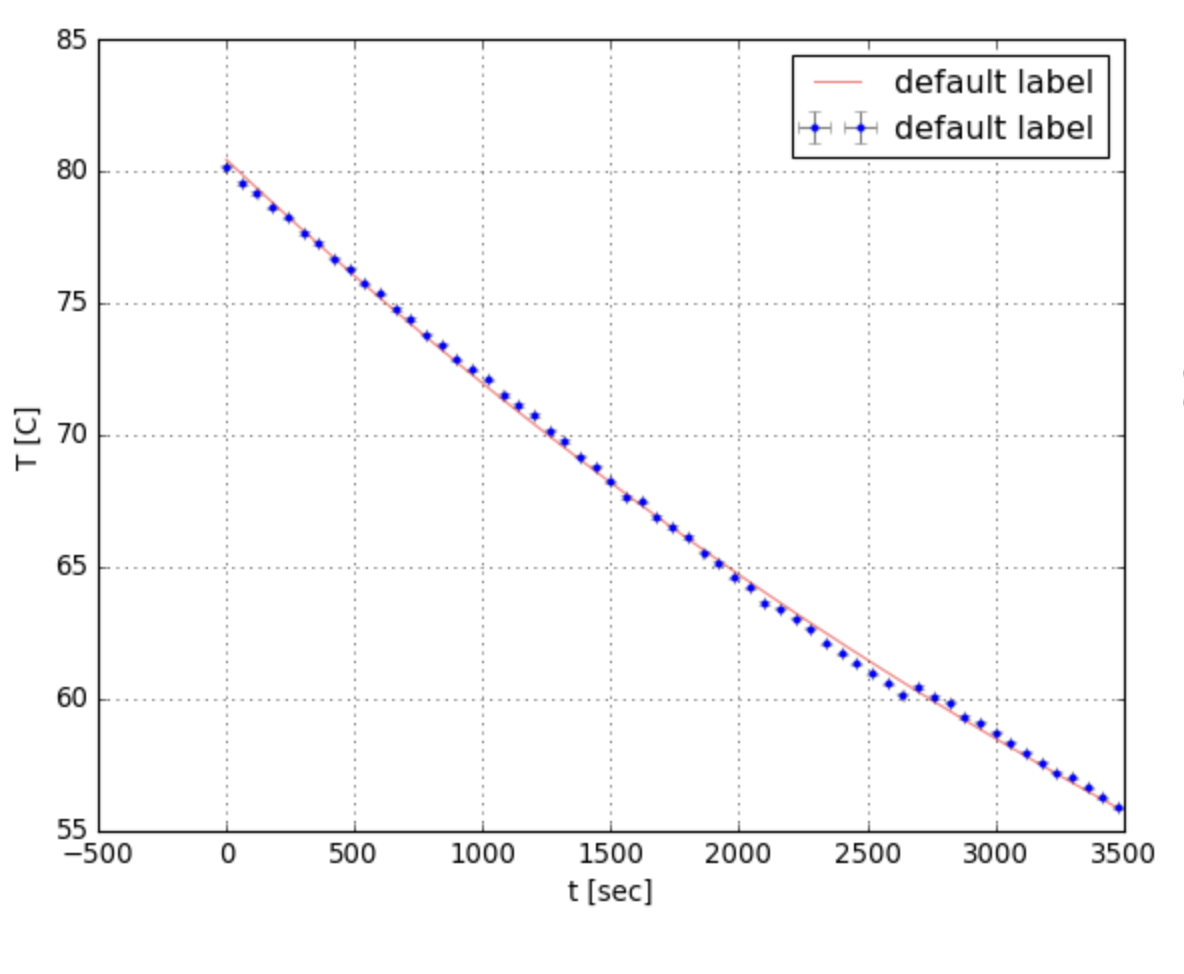
\includegraphics[width=\textwidth]{with lid/cooling fit.png}
      \caption{Exponential fit}
      \label{fig:with lid fit}
    \end{subfigure}
    \hfill
    \begin{subfigure}[b]{0.48\textwidth}
      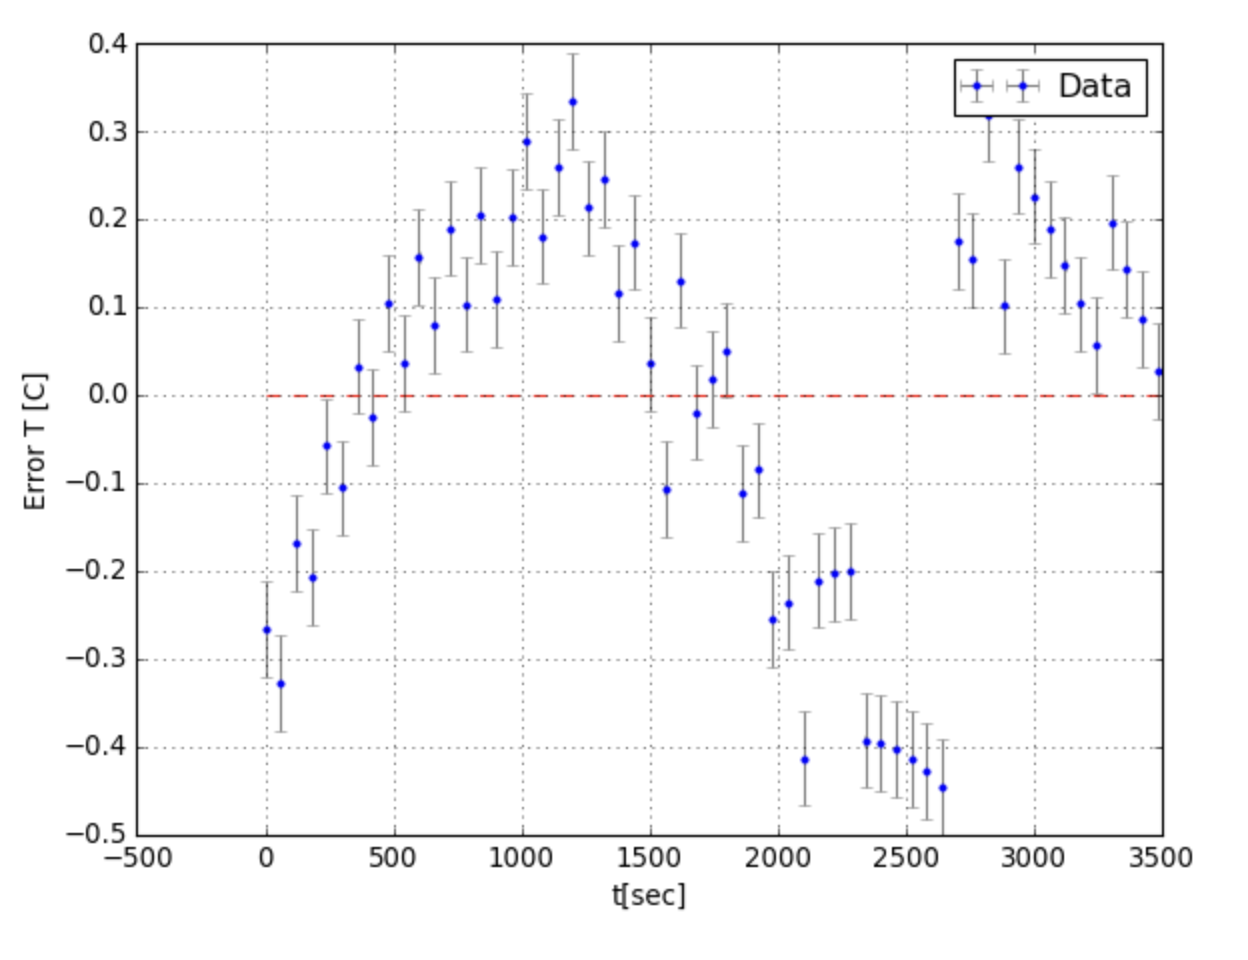
\includegraphics[width=\textwidth]{with lid/residuals fit.png}
      \caption{residual fit}
      \label{fig:with lid residual}
    \end{subfigure}
    \caption{with lid results}
\vspace{1em}
\begin{tabular}{ccccc}
\toprule
p‑probability & $\chi^2_{\mathrm{reduced}}$ & $a_0$ & $a_1$ & $a_2$ \\
\midrule
 $1.525 \cdot 10^{-165}$ & 17.20& $21.81 \pm 2.58$ & $58.642 \pm 2.52$ & $(156.22 \pm 8.93) \cdot 10^{-6}$ \\
\bottomrule
\end{tabular}
    \label{fig:risults with lid}
\end{figure}

As observed, the reduced chi-squared value ($\chi^2_{\mathrm{reduced}}$) is significantly greater than 1, suggesting that the model does not accurately capture all the experimental effects. Additionally, the very low p‑probability indicates that the measurement uncertainties might be underestimated or that additional systematic errors are present. The patterned behavior in the residuals further supports these observations and will be discussed in detail in the following section.
\pagebreak

and for the un-lidded measurments:

\begin{figure}[htbp]
    \centering
    \begin{subfigure}[b]{0.48\textwidth}
      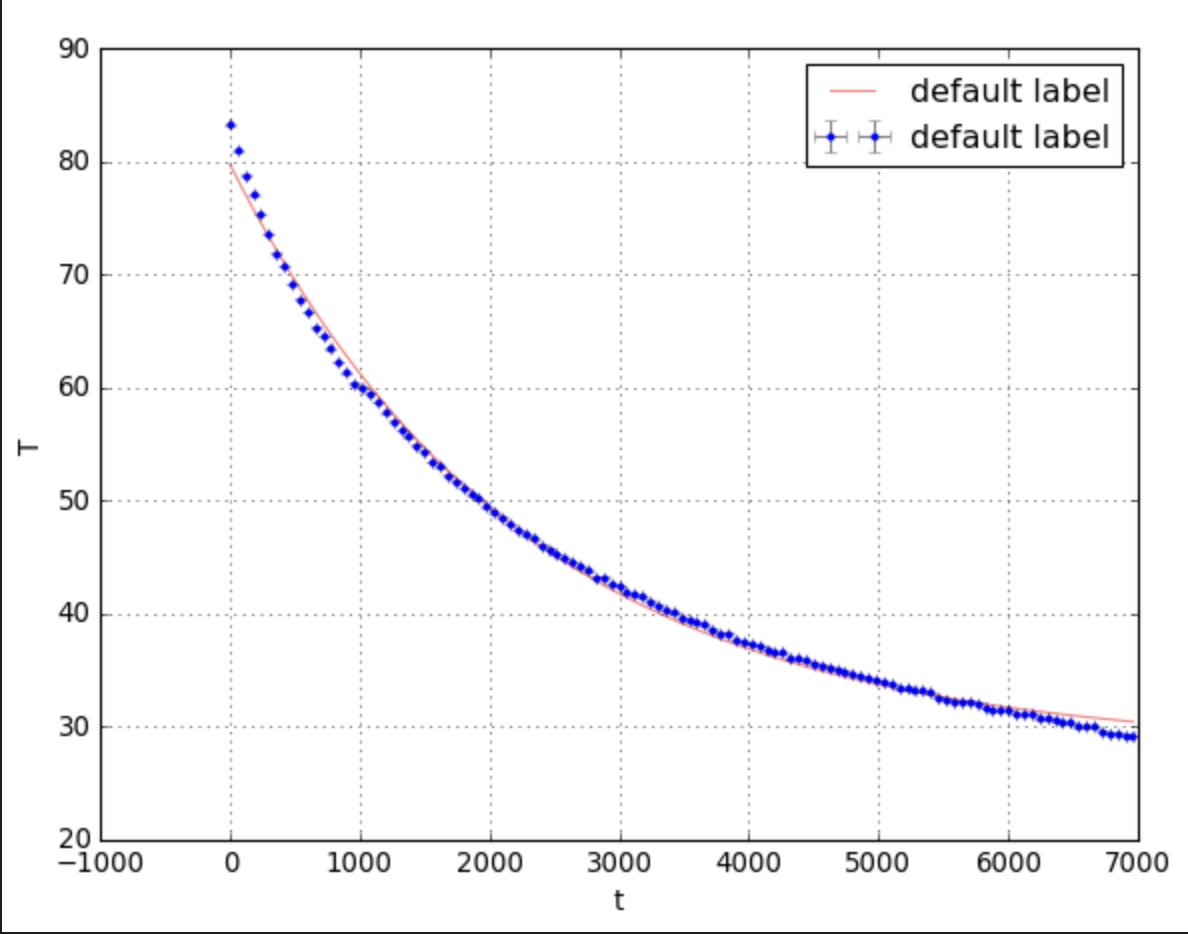
\includegraphics[width=\textwidth]{no lid/cooling fit.png}
      \caption{Exponential fit (no lid)}
      \label{fig:no lid fit}
    \end{subfigure}
    \hfill
    \begin{subfigure}[b]{0.48\textwidth}
      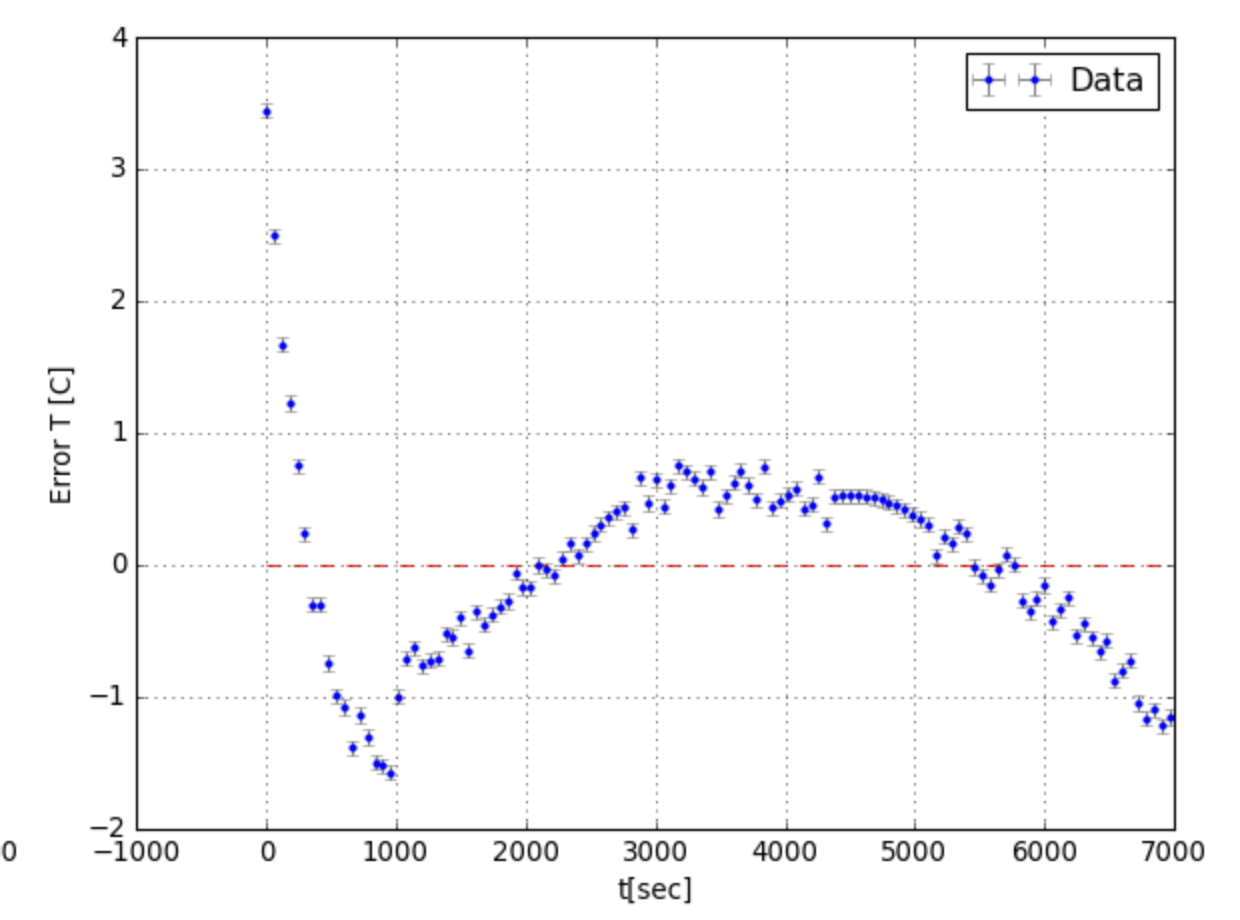
\includegraphics[width=\textwidth]{no lid/residuals fit.png}
      \caption{Residuals (no lid)}
      \label{fig:no lid residual}
    \end{subfigure}
    \caption{No lid results}
\vspace{1em}
\begin{tabular}{ccccc}
\toprule
p‑probability & $\chi^2_{\mathrm{reduced}}$ & $a_0$ & $a_1$ & $a_2$ \\
\midrule
 00 & $197.77$ & $27.94 \pm 0.25$ & $51.86 \pm 0.27$ & $(439.58 \pm 6.99) \cdot 10^{-6}$ \\
\bottomrule
\end{tabular}
    \label{fig:results no lid}
\end{figure}

Again, the high reduced chi-squared value and the near-zero p‑probability indicate that the model does not fully capture the experimental behavior. The residuals also exhibit systematic patterns, suggesting that additional effects or measurement uncertainties might be influencing the un-lidded results. In the next section, we further discuss these discrepancies
.

The calculated water heat transfer coefficient,
\[
h_{\mathrm{water}} = 62.57 \pm 12.40\,\mathrm{W/(m^2\,K)},
\]
falls significantly below the typical range of 600 to 3000 W/(m\(^2\)·K). This discrepancy suggests potential sources of error such as underestimated measurement uncertainties.

\section{Discution}
In summary, the experiment shows that the simple exponential cooling model captures the main trend of the water cooling, but it doesn’t include every detail of the process. The high reduced chi-squared values and near-zero p‑probabilities for both the lidded and un-lidded cases suggest that the measurement errors might be too low or that there are extra factors at work, like extra air currents or heat exchange with the environment.

The residual plots further illustrate this point. The systematic patterns observed in the residuals indicate that the model consistently under- or overestimates the cooling behavior during certain intervals. This non-random structure suggests that factors such as varying thermal contact, changes in ambient conditions, or unmodeled heat loss mechanisms might be influencing the experiment. In other words, while the exponential fit tracks the overall decay, the residuals reveal that the model does not capture all nuances of the physical process.

The measured water heat transfer coefficient is much lower than the typical range, which points to possible issues such as sensor calibration errors, imperfect insulation, or other factors influencing the cooling process. Even with these issues, the clear exponential decay in the logarithmic plots supports the idea behind Newton’s law of cooling.

Overall, this experiment shows that while the model captures the main trend, there are additional factors to consider. The activity demonstrates the basic concept of thermal relaxation and provides useful insights into how cooling systems work.



\end{document}



